% This work is licensed under the Creative Commons
% Attribution-NonCommercial 3.0 Unported License. To view a copy of this
% license, visit http://creativecommons.org/licenses/by-nc/3.0/.

\section{Aufbau} 

In diesem Versuch wird das \name{Stefan}-\name{Boltzmann} Gesetz
mithilfe eines Strahlungswürfels nach \name {Leslie} überprüft. Dieser
besitzt vier zu untersuchende Oberflächen, welche aus unterschiedlichen
Materialien bestehen und kann mit Wasser gefüllt werden. Die vier
verschiedenen Oberflächen sind eine weiß lackierte Fläche, eine schwarz
lackierte Fläche, eine matte Metallfläche und eine glänzende
Metallfläche.

Um die abgestrahlte Wärmeleistung zu untersuchen wird eine Thermosäule
nach \name{Moll} verwendet.  Diese besteht aus mehreren in Serie
geschalteten Thermoelementen. Die durch die Wärmeleistung entstehende
Thermospannung wird mit einem Voltmeter gemessen.

In Abb. \ref{fig:aufbau} ist eine schematische Darstellung der Versuchsapparatur zu sehen.
%
\begin{figure}
  \centering
  \includegraphics[width=0.8\textwidth]{aufbau.pdf}
  \caption{Schema der verwendeten Apparatur}
  \label{fig:aufbau}
\end{figure}
%
